\documentclass[conference]{IEEEtran}
\usepackage{cite}
\usepackage{amsmath,amssymb,amsfonts}
\usepackage{graphicx}
\usepackage{textcomp}
\usepackage{xcolor}
\usepackage{multicol}
\usepackage{float}
\usepackage[spanish]{babel}
\usepackage[spanish,vlined,ruled,]{algorithm2e}
\usepackage{hyperref}

\def\BibTeX{{\rm B\kern-.05em{\sc i\kern-.025em b}\kern-.08em
    T\kern-.1667em\lower.7ex\hbox{E}\kern-.125emX}}
\begin{document}

\title{Morphing}
\author{\IEEEauthorblockN{Joaquín Pérez Araya}
\IEEEauthorblockA{\textit{Departamento de Ciencias de la Computación} \\
\textit{Universidad de Chile}\\
Santiago, Chile \\
joaquin.perez.a@ug.uchile.cl}}


\maketitle

\begin{abstract}
	En este documento se aborda el tema del \textit{morphing}, una técnica de mezclado de imágenes la cual consiste en crear un proceso de metamorfosis entre una imagen y otra, adicionalmente se muestra una implementación realizada con resultados utilizando diferentes imágenes.
\end{abstract}
 

\section*{Introducción} % ***Así la cosa no me molesta con los numeritos***
	El \textit{morphing} es un tipo de efecto visual el cual se produce al cambiar una imagen a otra con un efecto de metamorfosis, actualmente se utiliza principalmente para el entretenimiento, en este documento se implementará el algoritmo descrito por Beier-Neely\cite{Paper}, que consiste en utilizar líneas de correspondencia entre la imagen de partida y la imagen de destino para describir la forma en que la mutación se va a llevar a cabo. El documento primero se describirá el diseño en la implementación, qué partes del algoritmo se implementaron y de qué forma, luego se probará éste código con diferentes dos muestras con distintos tipos de líneas para observar qué lineas son las mejores para este algoritmo. Para finalizar con las observaciones y conclusiones de dichos experimentos.
	
	
\section*{Diseño e Implementación}
	El código implementado define 3 funciones principales las cuales están implementadas en \texttt{morphing.py}: \textit{warp}, \textit{morph} y \textit{create morphing video}: La transformación de una imagen según un par de conjuntos de líneas (\textit{warp}), la creación de múltiples imágenes que son las que forman parte del morphing (\textit{morph}) y finalmente la creación, a partir de las imágenes calculadas en el proceso anterior el vídeo que muestra el cambio de las imágenes a lo largo del tiempo \textit{create morphing video}. También se dispone de un módulo adicional llamado \texttt{util.py} el cual contiene funciones auxiliares, tales como el cálculo de distancias y en general la aplicación de fórmulas detalladas en el artículo \cite{Paper}.
	
	\subsection*{Warpping}
		Para el \textit{warpping} se utiliza el algoritmo propuesto en el artículo\cite{Paper}, que está especificado en el Algoritmo 1, el cual crea una imagen vacía con las mismas dimensiones de la imagen fuente, y itera sobre ésta, calculando qué colores debería tener según las líneas de correspondencia y la imagen fuente.

	\begin{algorithm}[ht]
		\caption{Warpping}	
		\KwData{$image$ imagen fuente, $lines_{src}$ líneas fuente, $lines_{dst}$ líneas de destino.}
		\KwResult{Imagen que corresponde a la imagen fuente modificada según las líneas dadas.}
		\DontPrintSemicolon
	$destinationImage = zeros(shape(image)) $ \;
	\For{Pixel $X$ in $image$}{
		$DSUM = (0,0)$ \;
		$weightsum = 0$ \;
	\For{Line $P_i Q_i$ in $lines_{src}$ and $ P_i^{\prime} Q_i^{\prime}$ in $lines_{dst}$}{
	$u, v = calculate\_u\_v(X,P_i, Q_i)$ \;
	$X^\prime = calculate\_X^\prime (u,v,P_i^{\prime}, Q_i^{\prime})$ \;
	$D_i = X_i^\prime - X$		\;
	$weight = calculate\_weight(X, u, v, P_i, Q_i)$ \;
	$DSUM += D_i * weight$ \;
	$weightsum += weight$ \;
			}		
	$\bar{X} = X + DSUM / weightsum$
	$destinationImage(X) = image(\bar{X})$ \;		
		}
		\KwRet{$destinationImage$}
		\label{asdf}
		\end{algorithm} 

	La implementación usa el algoritmo en su versión \textit{inverse mapping}, es decir durante la ejecución se recorre la imagen de destino calculando qué pixeles de la imagen original deberían estar allí utilizando interpolación bilineal de los pixeles más cercanos de la imagen original, este método ofrece más simplicidad dado que se conoce los pixeles de destino de antemano por lo que el único inconveniente es el caso de que se requieren píxeles fuera de la imagen original por lo que se interpola según los pixeles ya calculados anteriormente, en cuyo caso sería:
		\begin{itemize}
               	\item Si se está en el primer pixel de la imagen, el de la esquina superior izquierda, éste se calcula como el pixel del mismo punto de la imagen de origen.
               	\item Si se está en la fila superior, se calcula usando el pixel anterior calculado, el de la izquierda de éste.
               	\item Si se está en la columna de la izquierda, se calcula usando el pixel de la fila superior.
               	\item Si se está en la columna de la derecha, se calcula utilizando los 3 pixeles que están cercanos a éste: Superior izquierdo, superior e izquierdo.
               	\item De otra forma se calcula utilizando 4 pixeles cercanos: Superior izquierdo, superior, superior derecho e izquierdo.
		\end{itemize}
	
		En el módulo de utilidades, están implementadas las funciones para el cálculo de $u$, $v$, $X^\prime$ y $weight$ según como se indica en el artículo.	Para los parámetros de cuanto peso tiene una línea respecto al punto se eligió: $A = 1, B = 1 $ y $ p= 0.5$. No hay ningún cambio respecto a la implementación de éstas formulas.
		
	
	\subsection*{Morphing y Video}
	Para la creación del conjunto de imágenes que forman el \textit{Morphing} completo se realiza lo siguiente: se itera por el número de imágenes $n$ que uno quiere incluir en el vídeo, se calcula el valor de entrelazado $t$ que va desde $0$ hasta $1$ de $1/n$ en $1/n$ pasos, según el grado de avance del Morphing. \\
	Dado un $t$ de éste proceso, para crear una imagen, se realiza un cross-fade entre dos imágenes: el \textit{warp} de la imagen fuente con sus líneas y la interpolación de las líneas fuente hacia las líneas de destino según $t$, es decir $t \cdot lines_{src} + (1 - t) \cdot lines_{dst}$, y el \textit{warp} entre la imagen de destino con sus líneas y la interpolación de las líneas de destino hacia las fuentes según $t$, que es $(1 - t) \cdot lines_{src} + t \cdot lines_{dst}$. Al final se añade a la colección de imágenes la ponderación de $t$ por la primera imagen más $1 - t$ de la segunda. \\
	
	Luego de finalizado la creación de la colección de imágenes del morphing, se utiliza la librería de OPENCV para formar un vídeo con éstas, en esta implementación, los vídeos generados están a 10 cuadros por segundo y en formato \texttt{.avi}.


\section*{Experimentación}
	Para verificar la precisión de la implementación, se utilizó un caso simple que consiste en transformar un círculo rojo en un cuadrado, una simple transformación. En la sección de Anexo se encuentra el detalle respecto a la obtención de este ejemplo.

	Se realizaron pruebas con dos pares de imágenes, donde se crearon las líneas a mano y después se ejecutaba el programa para revisar los efectos: Una con un par con dos felinos distinos, un puma y una leona, y la otra con un par de un mismo actor. Para prueba se crearon 3 conjuntos de líneas, uno con líneas de contorno (véase las líneas verdes en la figura 1), uno con líneas de expresión (las líneas azules en la misma figura) y por último uno con ambas líneas en conjunto.
	
\begin{figure}[H]
\begin{multicols}{2}
    \centering
    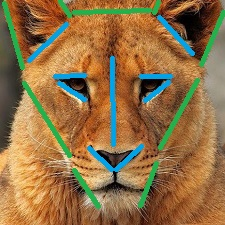
\includegraphics[height=0.65\linewidth]{cats/1 lines.jpg} \par
    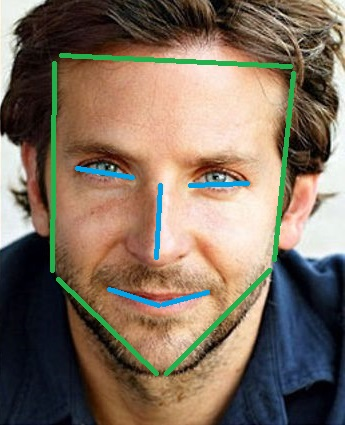
\includegraphics[height=0.65\linewidth]{faces/1 lines.jpg} \par
    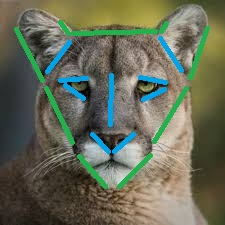
\includegraphics[height=0.65\linewidth]{cats/2 lines.jpg} \par
    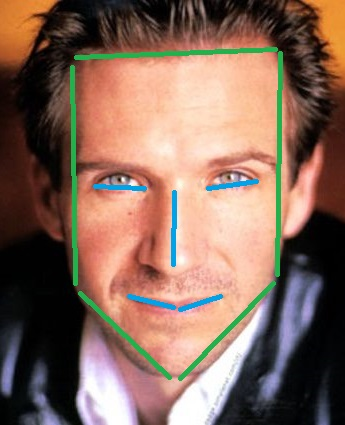
\includegraphics[height=0.65\linewidth]{faces/2 lines.jpg} \par
\end{multicols}
\caption{Imágenes usadas para la experimentación, están marcadas las líneas utilizadas para el Morphing, las verdes corresponden a contornos de la figura mientras que las azules corresponden a características intrínsecas de la imagen. Las imágenes de la izquierda corresponden a las de fuente mientras que las de la derecha corresponden a las de destino.}
\end{figure}
	
	Para cada prueba, se ejecutó la implementación requiriendo 50 imágenes en total, de las cuales, por motivos de simplicidad, sólo se presentarán la $1^{ra}, 10^{ma}, 20^{va}, 30^{va}, 40^{va}$ y $50^{va}$ imagen de dichas ejecuciones, sin embargo dentro del directorio de la implementación estarán las pruebas con sus respectivas imágenes y vídeos.
	De aquí en adelante, se mencionará como imágenes verdes, las imágenes que fueron creadas a partir del conjunto de líneas verdes, e imágenes azules de forma análoga. 


	\subsection*{Imágenes de Caras}
\begin{figure}[H]
\begin{multicols}{3}
    \centering
    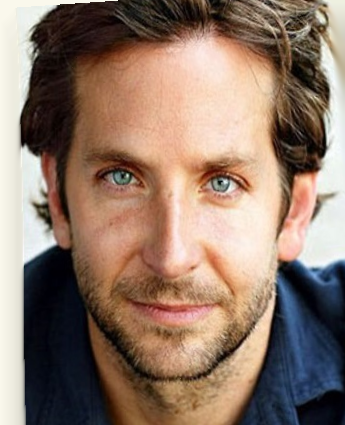
\includegraphics[width=1.0\linewidth]{results/faces/G/img01.png} \par
    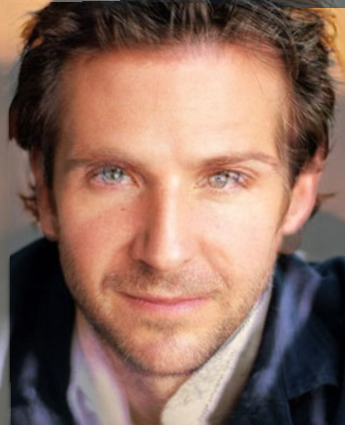
\includegraphics[width=1.0\linewidth]{results/faces/G/img30.png} \par
    
    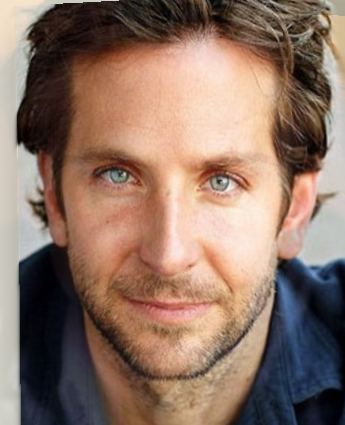
\includegraphics[width=1.0\linewidth]{results/faces/G/img10.png} \par
    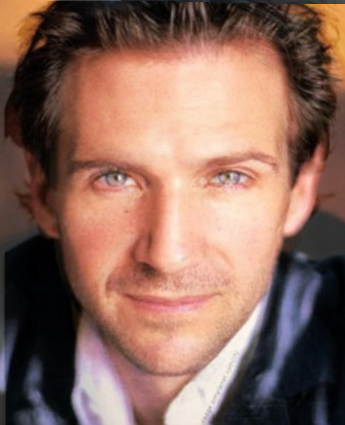
\includegraphics[width=1.0\linewidth]{results/faces/G/img40.png} \par

    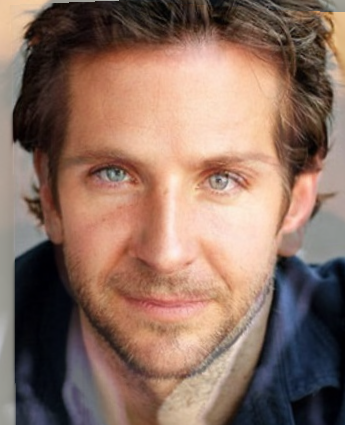
\includegraphics[width=1.0\linewidth]{results/faces/G/img20.png} \par
    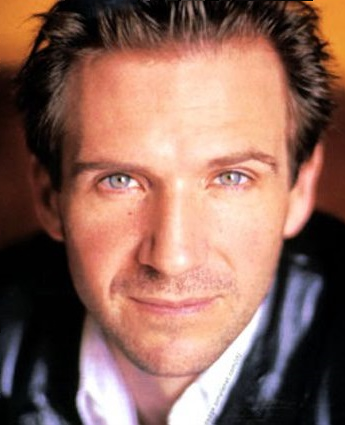
\includegraphics[width=1.0\linewidth]{results/faces/G/img50.png} \par
\end{multicols}
\caption{Imágenes creadas con la implementación y sólo las líneas verdes. El progreso va de izquierda a derecha de arriba hacia abajo.}
\end{figure}


\begin{figure}[H]
\begin{multicols}{3}
    \centering
    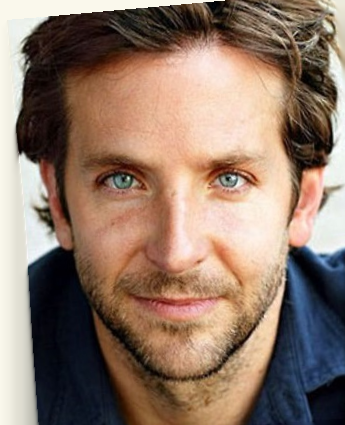
\includegraphics[width=1.0\linewidth]{results/faces/B/img01.png} \par
    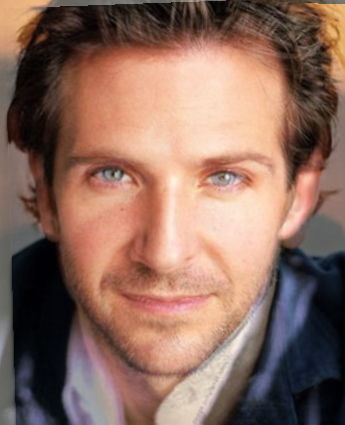
\includegraphics[width=1.0\linewidth]{results/faces/B/img30.png} \par
    
    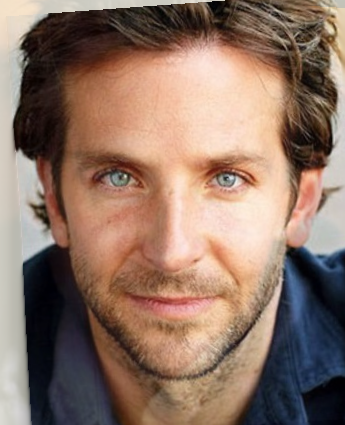
\includegraphics[width=1.0\linewidth]{results/faces/B/img10.png} \par
    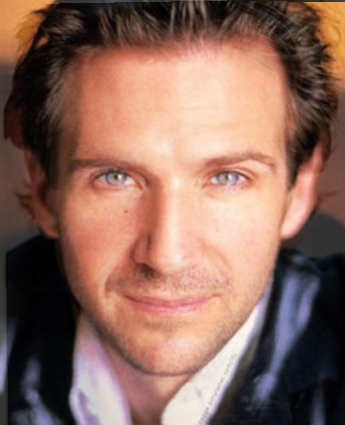
\includegraphics[width=1.0\linewidth]{results/faces/B/img40.png} \par

    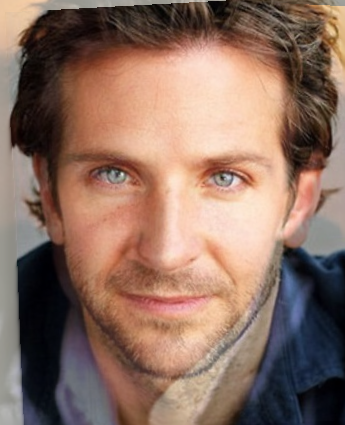
\includegraphics[width=1.0\linewidth]{results/faces/B/img20.png} \par
    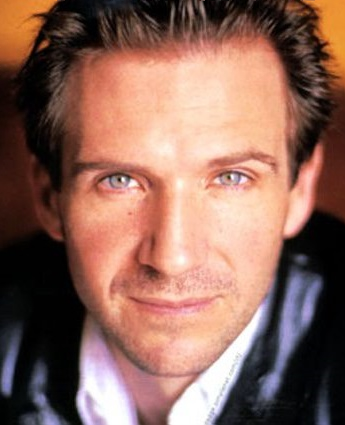
\includegraphics[width=1.0\linewidth]{results/faces/B/img50.png} \par
\end{multicols}
\caption{Imágenes creadas con la implementación y sólo las líneas azules. El progreso va de izquierda a derecha de arriba hacia abajo.}
\end{figure}

\begin{figure}[H]
\begin{multicols}{3}
    \centering
    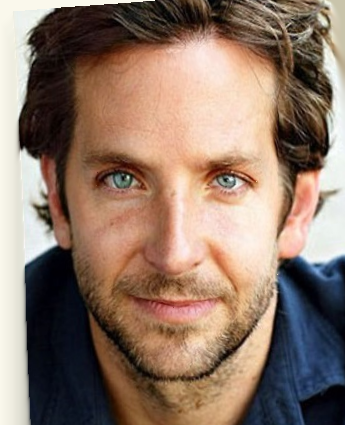
\includegraphics[width=1.0\linewidth]{results/faces/XL/img01.png} \par
    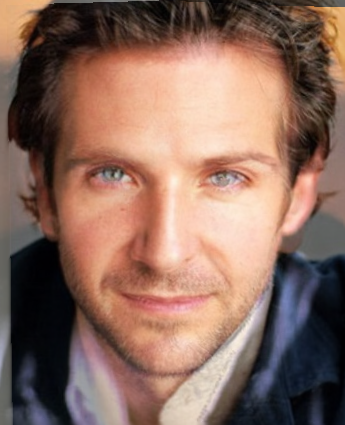
\includegraphics[width=1.0\linewidth]{results/faces/XL/img30.png} \par
    
    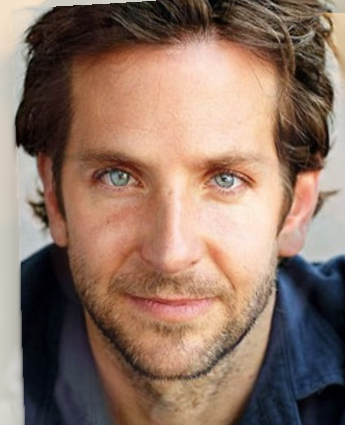
\includegraphics[width=1.0\linewidth]{results/faces/XL/img10.png} \par
    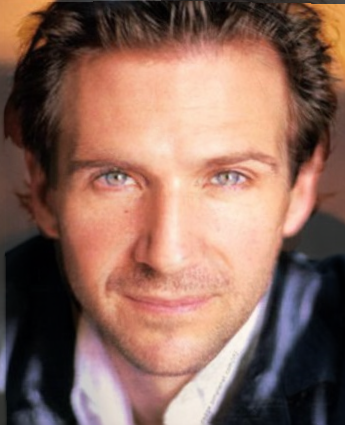
\includegraphics[width=1.0\linewidth]{results/faces/XL/img40.png} \par

    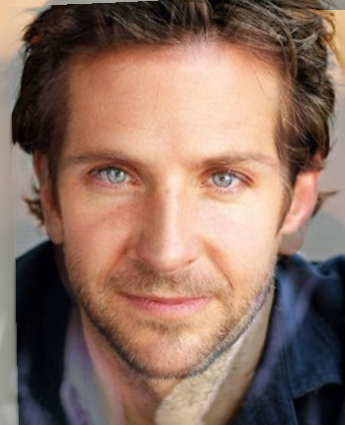
\includegraphics[width=1.0\linewidth]{results/faces/XL/img20.png} \par
    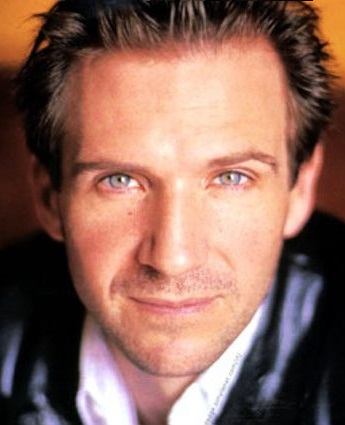
\includegraphics[width=1.0\linewidth]{results/faces/XL/img50.png} \par
\end{multicols}
\caption{Imágenes creadas con la implementación y con ambos pares de líneas. El progreso va de izquierda a derecha de arriba hacia abajo.}
\end{figure}

	En este caso, el conjunto que trae mejores resultados visuales es el Verde, dado que las líneas azules producen tanto cuando se usan solas y combinadas un mal efecto de transición en los ojos de la imagen, quedando meramente como sólo un fade. Y como se discutirá más adelante en la sub-sección de errores, la elección de las líneas no fue sencillo.


	\subsection*{Imágenes de Felinos}
\begin{figure}[H]
\begin{multicols}{3}
    \centering
    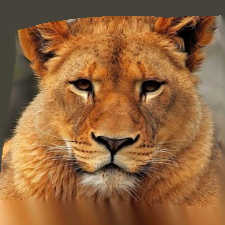
\includegraphics[width=1.0\linewidth]{results/cats/G/img01.png} \par
    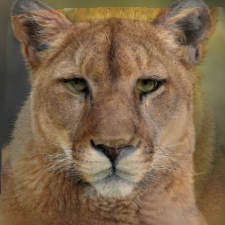
\includegraphics[width=1.0\linewidth]{results/cats/G/img30.png} \par
    
    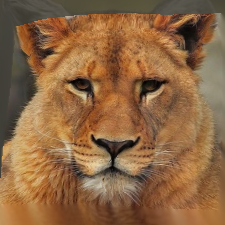
\includegraphics[width=1.0\linewidth]{results/cats/G/img10.png} \par
    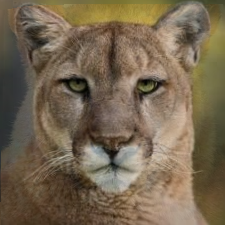
\includegraphics[width=1.0\linewidth]{results/cats/G/img40.png} \par

    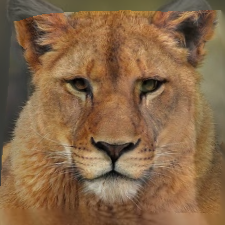
\includegraphics[width=1.0\linewidth]{results/cats/G/img20.png} \par
    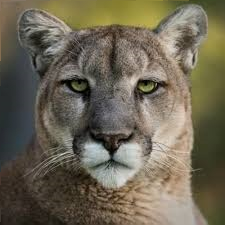
\includegraphics[width=1.0\linewidth]{results/cats/G/img50.png} \par
\end{multicols}
\caption{Imágenes creadas con la implementación usando sólo las líneas verdes. El progreso va de izquierda a derecha de arriba hacia abajo.}
\end{figure}

\begin{figure}[H]
\begin{multicols}{3}
    \centering
    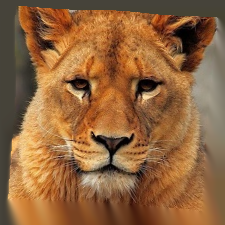
\includegraphics[width=1.0\linewidth]{results/cats/B/img01.png} \par
    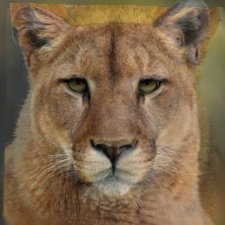
\includegraphics[width=1.0\linewidth]{results/cats/B/img30.png} \par
    
    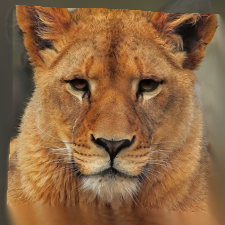
\includegraphics[width=1.0\linewidth]{results/cats/B/img10.png} \par
    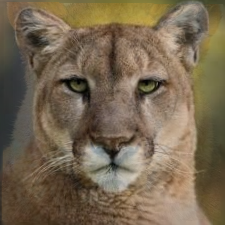
\includegraphics[width=1.0\linewidth]{results/cats/B/img40.png} \par

    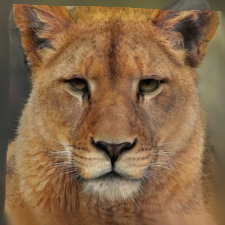
\includegraphics[width=1.0\linewidth]{results/cats/B/img20.png} \par
    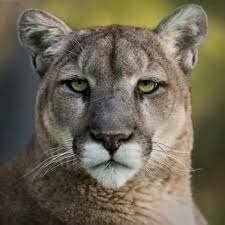
\includegraphics[width=1.0\linewidth]{results/cats/B/img50.png} \par
\end{multicols}
\caption{Imágenes creadas con la implementación usando sólo las líneas azules. El progreso va de izquierda a derecha de arriba hacia abajo.}
\end{figure}

\begin{figure}[H]
\begin{multicols}{3}
    \centering
    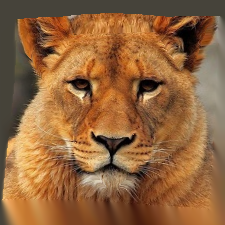
\includegraphics[width=1.0\linewidth]{results/cats/XL/img01.png} \par
    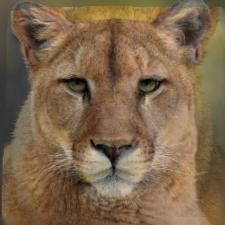
\includegraphics[width=1.0\linewidth]{results/cats/XL/img30.png} \par
    
    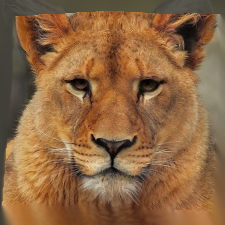
\includegraphics[width=1.0\linewidth]{results/cats/XL/img10.png} \par
    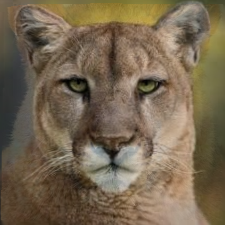
\includegraphics[width=1.0\linewidth]{results/cats/XL/img40.png} \par

    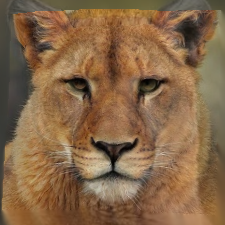
\includegraphics[width=1.0\linewidth]{results/cats/XL/img20.png} \par
    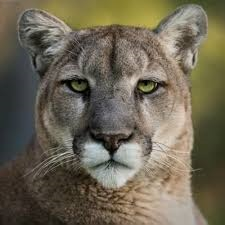
\includegraphics[width=1.0\linewidth]{results/cats/XL/img50.png} \par
\end{multicols}
\caption{Imágenes creadas con la implementación usando todas las líneas. El progreso va de izquierda a derecha de arriba hacia abajo.}
\end{figure}
	
	Con el conjunto de imágenes obtenidas con los diferentes experimentos se observa que en las imágenes creadas usando las líneas verdes (de contorno), la imagen inicial se dobla para hacer calzar las orejas de ambos felinos, creando así una aparcición de las orejas más armoniosa que en el caso de las imágenes creadas utilizando sólo las líneas azules, sin embargo, el conjunto de imágenes verdes presenta discordancias con las facciones de la cara de los felinos, éstas son más aparentes en la cuarta imagen (la primera de la segunda fila), donde se evidencian éstas en ojos y en nariz. Estos dos detalles no están presentes en las imágenes que usan todas las líneas.


	\subsection*{Errores}
	
	Durante el desarrollo de los experimentos empezaban se obtuvieron resultados dignos de notar y mostrar:
		

\begin{figure}[H]
\begin{multicols}{3}
    \centering
    
    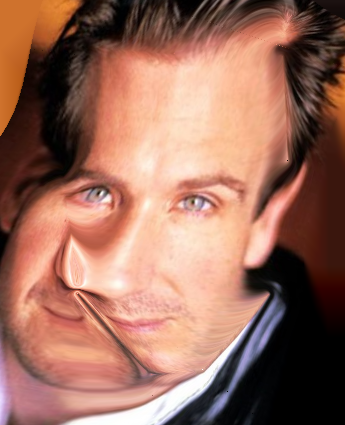
\includegraphics[width=0.65\linewidth]{extra/errors/02/img01.png} \par
    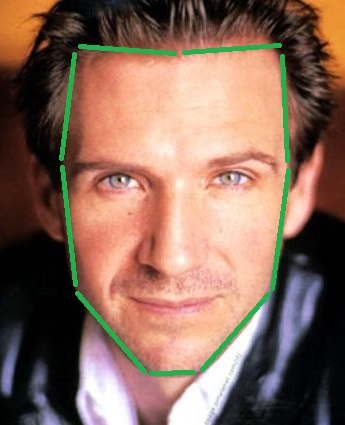
\includegraphics[width=0.65\linewidth]{extra/errors/02/1 lines.jpg} \par 
    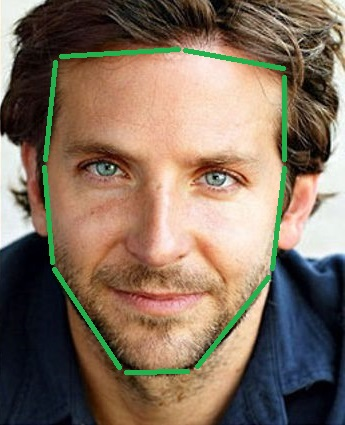
\includegraphics[width=0.65\linewidth]{extra/errors/02/2 lines.jpg} \par
   
\end{multicols}
\caption{Morphing creado con las imagenes y líneas de la derecha a ésta.}
\end{figure}	

	Se puede evidenciar en el anterior ejemplo, que existe la necesidad de utilizar una cantidad mínima de líneas para indicar una mismo sector. Dado que el alto número de líneas para describir el borde de ambas caras causa altas anomalías.
	
	Dentro de la experimentación queda en evidencia que la elección de líneas no es trivial, considerando la figura, ahí que la elección de líneas muy cercanas entre unas y otras afectan gravemente determinadas zonas, en el caso de la figura anterior la zona de los ojos.
		

\begin{figure}[H]
\begin{multicols}{3}
    \centering
    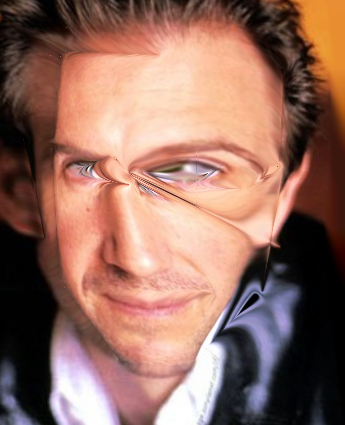
\includegraphics[width=0.65\linewidth]{extra/errors/01/img01.png} \par
    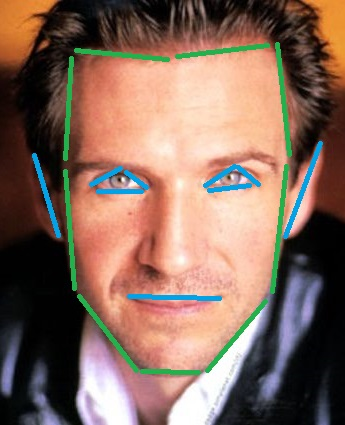
\includegraphics[width=0.65\linewidth]{extra/errors/01/1 lines.jpg} \par
    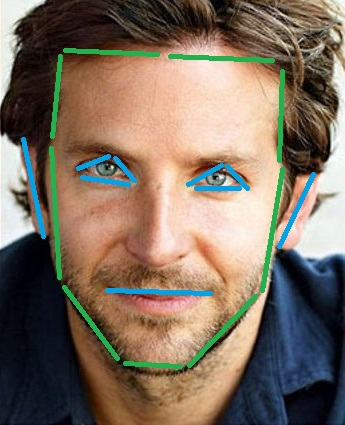
\includegraphics[width=0.65\linewidth]{extra/errors/01/2 lines.jpg} \par
   
\end{multicols}
\caption{Morphing creado con las imagenes y líneas de la derecha a ésta.}
\end{figure}	
	
	Estos errores permitieron realizar una mejor selección de líneas para las pruebas mostradas en la primera parte de esta sección.

\section*{Conclusión}
	El uso de líneas de contorno (verdes) tiende a ser más efectivo al momento de usar \textit{morphing} en caras que el uso de líneas de características (azules), sin embargo la falta de líneas características puede  crear defectos visuales al momento de crear una animación. Por lo que es recomendable usar líneas de contorno para la figuras más una cantidad mínima de líneas de características.
	No es trivial la elección de líneas para la ejecución del proceso de \textit{morphing}, si se elige de forma errónea o usando muchas líneas pueden ocurrir errores como los vistos en la sección de experimentación, también el uso desmedido de líneas provoca que el tiempo de ejecución sea mucho más alto, por lo que reduce increíblemente el rendimiento, por lo que esta técnica sería más útil implementarla en lenguajes compilados como C o Java, así se podría ejecutar el algoritmo en tiempos menores, dado que en la implementación actual, crear la animación de las imágenes toma alrededor de una hora o más.

\section*{Bonus}
	Durante el proceso de creación de este trabajo, se encontraron ejemplos extra con sus líneas incluídas. Dado que no eran lo pedido como tarea, no fueron incluídos dentro de la experimentación, pero vale la pena mencionarlos, en la carpeta extra, del directorio del código se encuentran dos casos encontrados en internet:
	\begin{itemize}
	\item Dos imágenes de caras que son las caras que se estudian en el artículo del algoritmo implementado, contiene dos conjuntos de líneas, uno con 30 líneas y el otro con una cantidad abismal de líneas (42), al ser poco eficiente la implementación, ¡la ejecución del conjunto de líneas más grande toma alrededor de 8 horas!. Esta fue obtenido de \url{https://www.cs.toronto.edu/~mangas/teaching/320/assignments/a4}, que está dentro del código para la revisión de la tarea dada.
	\item Un círculo y un cuadrado, este caso se utilizó para verificar la implementación dado que sólo contiene dos líneas, es simple para verificar los errores de ejecución. Este fue obtenido de \url{http://cns.bu.edu/~oph/cs580_assign1/p1.html}.
	
	\end{itemize}

		
	
\begin{thebibliography}{99}
	 \bibitem{Paper} T. Bier, S. Neely. Feature-Based Image Metamorphosis, Computer Graphics 1992-07

\end{thebibliography}

\end{document}

\begin{figure}[H]
    \centering
    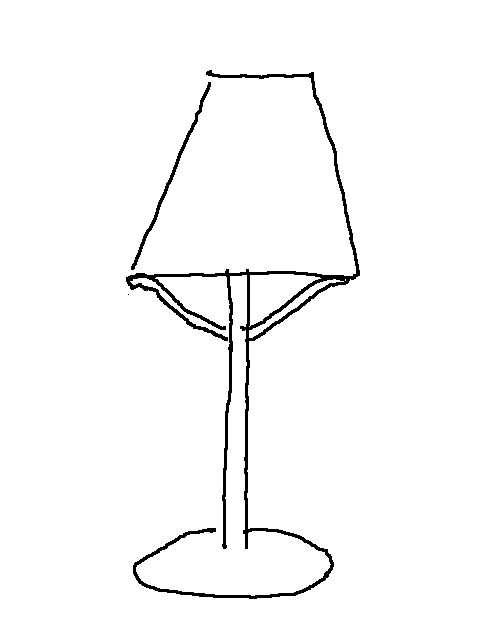
\includegraphics[width=0.95\linewidth]{image/lamps.jpg} \par

\caption{Ejemplo de una posible búsqueda, la imagen de la izquierda representa el dibujo de búsqueda y las de la derecha los resultados esperados.}
\end{figure}
